\chapter*[Introduction]{Introduction : intérêt de \LaTeX{} en sciences humaines et sociales}

\section{Un manque important}

Ce livre est le fruit d'un an de travail et d'utilisation quotidienne de \LaTeX pour la rédaction de mon mémoire de master. Il vient à mes yeux combler un vide. En effet si les ouvrages sur \LaTeX sont nombreux, rares sont ceux destinés  spécifiquement aux sciences humaines et sociales. 

Si le mot \LaTeX a déjà été entendu par des oreilles humanistes, il évoque -- sauf rares exceptions --- au mieux un outil pour les sciences dites dures, au pire la sève d'un arbre ou un plastique aux nombreuses applications. 

De nombreuses raisons pourraient expliquer ce quasi-vide.
\begin{itemize}
\item la tendance générale des chercheurs en sciences humaines à mal connaître ou méconnaître l'outil informatique ;
\item le fait que \LaTeX paraît \emph{au premier abord} peu convivial ;
\item le fait que pendant longtemps \LaTeX ne disposait pas d'outils pour gérer convenablement et simplement une bibliographie selon les normes propres aux sciences humaines : notes de bas de page, distinction entre sources primaires et secondaires etc ;
\item le fait que pendant longtemps la gestion des caractères non latins n'était pas des plus aisés en \LaTeX ;
\item le fait que les éditeurs de sciences humaines prennent rarement des textes formatés en \LaTeX parce que les auteurs les rédigent rarement en \LaTeX parce que les éditeurs les prennent rarement en \LaTeX \ldots
\end{itemize}

Alors que les chercheurs en sciences humaines sont des spécialistes de l'écrit, pendant longtemps seuls des logiciels de traitement de textes comme OpenOffice.org ou Microsoft Word ont été utilisés pour la rédaction des travaux universitaires.

Et c'est là un paradoxe : en effet, comme nous le verrons, ces traitements de texte souffrent de deux défauts majeurs qui devraient inciter les écrivains à changer :
\begin{itemize}
\item Ils produisent une typographie de médiocre qualité. Certes un chercheur ne publie pas lui-même ses travaux mais passe en général par un éditeur. Pour autant, l'apprentissage de la recherche commence par un mémoire de master, puis par une thèse, que l'étudiant édite lui-même pour les soumettre à son jury. Et de même qu'un travail manuscrit écrit lisiblement gagne la sympathie de son correcteur\footnote{Combien de fois n'ai-je pas perdu de points pour \enquote{graphie illisible} ?},  une typographie correcte rend la lecture plus agréable.
\item Leur module de gestion bibliographique manque de souplesse. Je ne connais personne qui m'ait déclaré êtres satisfaits de ceux livrés en standard avec leur traitement de texte.
\end{itemize}

\section{Pourquoi \LaTeX{} ?}

\subsection{Inconvénient des traitements de textes}

Quand vous rédigez un texte dans votre traitement de texte, comme par exemple Microsoft Word ou Openoffice.org, celui-ci exécute deux actions simultanées :

\begin{itemize}
\item D'une part il stocke dans un fichier la structure logique de votre texte : titres, paragraphes, notes de bas de pages etc.
\item D'autre part il vous affiche à l'écran le rendu \enquote{physique} de votre texte (justifications, gras, italiques etc), tel qu'un lecteur en disposera.
\end{itemize}

Pour cette raison on appelle ce type de logiciel WYSIWYG, ce qui en anglais est l'acronyme de  \textenglish{What You See Is What You Get}\footnote{\enquote{Ce que vous voyez est ce que vous faites}.}. 

Cette combinaison de deux fonctions différentes dans les  traitements de texte a trois conséquences :

\begin{itemize}
\item La nécessité d'afficher en temps réel le rendu physique du texte tout en conservant une vitesse relativement élevée du logiciel entraîne une baisse de la qualité typographique. Par exemple :
	\begin{itemize}
		\item Pour avoir un texte justifié à gauche et à droite, les traitements de texte font varier la taille des espaces entre les mots. Les variations peuvent parfois être considérables ce qui peut diminuer le confort de lecture. Pour éviter ce type d'ennui, les livres \enquote{classiques} coupent les mots en fin de ligne, ce qu'on appelle une césure\footnote{La césure ne se fait toutefois pas n'importe où : elle doit respecter des règles propres à chaque langue.}.
		\item Les blancs situés avant certains signes de ponctuations, comme par exemple les points d'exclamation sont de  la même taille que les blancs séparant les mots, alors que les règles typographiques \enquote{classiques} prévoient des blancs plus petits.
	\end{itemize}
\item Le fait qu'un même logiciel s'occupe \emph{à la fois} de l'affichage et de la structure du texte incite à confondre les deux\footcite[L'auteur de ces lignes est moins sévère envers les traitements de texte que d'autres LaTeXiens : \cf][]{stupide}  :
	\begin{itemize}
		\item Cela incite à se concentrer sur le forme plutôt que sur le fond et la structure\footcite[Toutefois en théorie la formation universitaire de sciences humaines incite à penser \emph{structure et sens d'abord}. Voir un débat sur le blog de l'auteur :][]{structurevsforme}. 
		\item Les rédacteurs n'utilisent pas toujours la possibilité de séparer sens et forme grâce aux styles. Dans ce cas, lorsqu'on désire changer la forme d'un élément logique (comme  le titre d'un chapitre) on doit changer l'ensemble des endroits où cet élément logique est utilisé\footnote{Par exemple, pour une personne  qui n'aurait pas utilisé les styles pour désigner ses titres de chapitre, il faudra sélectionner \emph{l'ensemble des titres de chapitres} puis aller dans les menus de mise en forme etc.}.
	\end{itemize}

\item Les lourds calculs informatiques nécessaire au calcul de la mise en forme en temps réel rendent les traitements de textes particulièrement lents comparativement à d'autres logiciels. Cette lenteur est souvent source d'énervement et de pertes de concentration. En outre, ces logiciels exigent bien souvent du matériel récent.
\end{itemize}

Par ailleurs, si les traitements de textes récents disposent d'outils de gestions de bibliographies, ceux-ci manquent en général de souplesse c'est pourquoi ils sont rarement utilisés. Ainsi nombreux sont les auteurs à écrire directement leur bibliographie \enquote{à la main} en tapant directement : Nom de l'Auteur, \emph{Titre}, etc. En cas d'erreur, il faut donc corriger l'ensemble des endroits où l'œuvre est citée.

\subsection{Avantage de \LaTeX{}}

\LaTeX{} permet de résoudre l'ensemble des problèmes des traitements de texte. En effet, \LaTeX{} sépare deux étapes : 

\begin{itemize}
\item L'étape de rédaction, qui se passe dans un éditeur de texte. L'auteur frappe son texte et indique par un certain nombre de commandes sa structure (titres, paragraphes, notes de bas de pages).
\item L'étape de calcul de l'affichage se fait seulement ensuite : l'auteur fait passer son fichier par un compilateur\footnote{Qu'on peut sommairement décrire comme un ensemble de scripts informatiques destinés à produire un objet informatique à partir d'un langage plus facile à lire pour les humains.}, parfois aussi appelé \emph{compositeur}. Ce dernier programme va lire l'ensemble des commandes du fichier pour produire un nouveau fichier au format \ext{pdf}\footnote{Historiquement \LaTeX{} produisait un autre format de fichier : \ext{dvi}. Mais pour notre propos, cela n'a pas d'importance : dans ce livre nous n'utiliserons que la production de \ext{pdf}.}.
\end{itemize}

Cette séparation permet :
\begin{itemize}
\item Une qualité typographique supérieure :  le compositeur n'étant pas contraint par la nécessité d'un affichage en temps réel, il peut faire des calculs plus lourds : ainsi par exemple \LaTeX{} produit des césures typographiques et non pas des blancs à géométrie variable, et équilibre bien mieux la composition du texte.
\item Une meilleure séparation du sens et de la forme puisque l'auteur donne uniquement des indications de sens.
\end{itemize}

En outre \LaTeX{} possède un système de gestion de la bibliographie extrêmement puissant. Il permet à l'auteur de séparer le contenu de sa bibliographie\footnote{Titres, auteurs etc.} de son affichage\footnote{Faut-il mettre des \emph{op. cit.}, et si oui où ; faut-il mettre uniquement les initiales des prénoms ou les prénoms en entier etc.}.

Cette séparation entre contenu de la bibliographie et affichage est utile non seulement aux auteurs mais aussi aux éditeurs. En effet, si l'auteur structure correctement sa base de donnée bibliographique\renvoi{bddbiblio} l'éditeur peut adapter l'affichage de la bibliographie à ses propres règles : il lui suffit de créer des fichiers de styles bibliographiques qui suivent une syntaxe simple.

La gestion d'une bibliographie est à la fois l'un des travaux les plus importants en sciences humaines \emph{et} l'un des plus pénibles, avec des nombreuses sources possibles d'erreurs. Cette simple raison suffit aux yeux de l'auteur à préférer \LaTeX{} à un logiciel de traitement de texte\footnote{L'auteur ainsi que sa sœur se sont décidés à utiliser \LaTeX{} dans le cadre de leurs travaux universitaires, et l'élément déclencheur du choix a été la facilité et la souplesse de la gestion bibliographique.}.

Un autre avantage de \XeLaTeX{} est la production directe d'un document au format PDF. Lorsque l'on reçoit des documents sous forme numérique, il est bien fréquent qu'à l'ouverture du fichier la mise en page soit perdue, que l'impression soit de mauvaise qualité, ou même qu'il soit tout bonnement impossible d'ouvrir le fichier.

Le \emph{Portable Document Format} permet de pallier à ces inconvénients. Il s'agit d'un format \emph{ouvert}, c'est-à-dire que son créateur, la société Adobe, a publié toutes les spécifications nécessaires à la création de logiciels pouvant lire ce format. Par conséquent, il existe de nombreux lecteurs de PDF utilisables sur un grand nombre de systèmes d'exploitations\footnote{Pour un aperçu des lecteurs libres et gratuits disponibles pour votre système d'exploitation si vous n'en disposez pas déjà d'un, rendez-vous à la page \url{http://pdfreaders.org/index.fr.html} (en français).}.

Le format PDF est conçu pour être lisible de manière universelle. Il embarque en effet dans un même fichier non seulement le texte et les éventuelles images, mais aussi les indications de mise en page et les polices de caractères. Être aussi complet vous garanti que celui qui visionnera votre document ou bien le lira sous sa forme imprimée verra exactement ce que \emph{vous} aviez en tête lorsque vous l'avez composé, ce qui constitue un avantage indéniable sur les formats de fichiers tels que celui de Microsoft Word, par exemple. En outre, vous avez la certitude que le PDF que vous conservez est pérenne. Dans la mesure où chacun est libre de concevoir un logiciel permettant la lecture des PDF et que les spécifications sont librement accessibles, vous avez la garantie de ne pas voir le sort de vos publications dépendre de la bonne volonté d'un vendeur de logiciels au cours des années à venir, ce qui fait du PDF un format de choix pour archiver des publications.

La médaille a hélas son revers: format de fichier lisible universellement, le PDF est fort difficile à modifier confortablement: il n'est pas prévu pour cet usage. C'est pourquoi, si vous souhaitez travailler en collaboration sur un ouvrage en utilisant \XeLaTeX{}, il vous faudra travailler différemment.\renvoi{travail collaboratif}

\subsection{Qu'est qu'un éditeur de texte ?}

J'ai parlé dans les paragraphes précédents de deux types de logiciels, qu'il ne faut pas confondre :
\begin{itemize}
	\item Les traitements de texte.
	\item Les éditeurs de texte.
\end{itemize}

Nous avons vu ce qu'étaient les premiers : des logiciels qui s'occupent d'insérer dans un fichier la structure logique d'un texte \emph{et} de montrer son rendu physique.
Les seconds sont simplement des logiciels qui permettent à une personne d'écrire dans un fichier texte et de placer lui même ses commandes de structurations.
Toutefois les bons éditeurs de texte font plus que cela : ils aident à sa rédaction par différents outils :
\begin{itemize}
\item Souvent ils colorient à l'écran les commandes, afin de permettre de mieux les visualiser; c'est ce que l'on appelle la coloration syntaxique.
\item Ils proposent des raccourcis pour taper les commandes les plus fréquentes :  raccourcis clavier, boutons etc.
\item Ils proposent parfois un affichage du plan du travail.
\end{itemize}

Certains de ces éditeurs de texte sont généralistes et adaptés à plusieurs langages informatiques\footnote{Par exemple le \LaTeX{} et le HTML, ce dernier étant utilisé pour les sites internet.}. D'autres sont spécialisés dans tel ou tel langage : ils proposent en général des outils supplémentaires propres au langage de spécialisation. 

Ainsi les éditeurs spécialisés en \LaTeX{} proposent des boutons spécifiques afin de lancer le compositeur \LaTeX{}.

Pour commencer en \LaTeX{} il vous faudra donc abandonner votre ancien traitement de texte et choisir un éditeur de texte spécialisé en \LaTeX{} : nous en listons plusieurs en annexe\renvoi{annexe:editeurs}.

\section[TeX, LaTeX, XeTeX, XeLaTeX : points communs et différences]{\TeX{}, \LaTeX{}, \XeTeX{} et \XeLaTeX{} : points communs et différences}\label{TeXLaTeX}

Dans ce chapitre nous avons parlé de \LaTeX{}. Le titre de ce livre parle pourtant  de \XeLaTeX{}. Quelle est la différence ? Voici une brève explication historique, très simplifiée\footnote{Le lecteurs curieux trouvera aisément de la documentation plus détaillée sur le sujet.}.

\begin{enumerate}
\item En 1977 Donal Knuth invente  \TeX{} qui était un simple compositeur de texte, capable de transformer un texte structuré par des commandes en un texte mis en forme. Avec \TeX{} on pouvait également inventer ses propres commandes.
\item L'utilisation de \TeX{} était relativement complexe. Leslie Lamport a créé un ensemble de commandes \TeX{} pour en simplifier l'usage. Cet ensemble de commande a permis de former le langage \LaTeX{} et le compositeur associé.
\item Par la suite un compositeur dérivé de \TeX{} a été créé : \XeTeX{}. Ce compositeur permet deux choses :
\begin{itemize}
	\item Une gestion  de l'ensemble des écritures mondiales, par le biais du jeu de caractères Unicode\renvoi{utf8}.
	\item Une gestion des nouvelles polices de caractères au format OpenType\footnote{Ce type de fonte permet, par exemple, une gestion poussée des ligatures entre les caractères.}, apparus au début des années 2000.

\end{itemize} 
\item Pour permettre d'utiliser les commandes de \LaTeX{} avec \TeX{} on a créé \XeLaTeX{}.
\end{enumerate}

On peut résumer les liens entre \TeX{}, \LaTeX{}, \XeTeX{} et \XeLaTeX{} par le schéma \ref{sch:tex} (p. \pageref{sch:tex}).

\begin{figure}[ht]
\centering
% Schéma des parentes entres TeX LaTeX XeTeX etc.
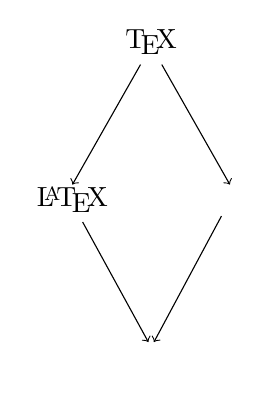
\begin{tikzpicture}
	
	% Les textes
	\node[text height=1ex,anchor=mid] (T) at (0,0) 		 	{\TeX} ;
	\node[text height=1ex,anchor=mid]  (X) at (1, -2)	 	 	{\XeTeX};
	\node[text height=1ex,anchor=mid]  (L) at (-1, -2) 		{\LaTeX};
	\node[text height=1ex,anchor=mid]  (XL) at (0,-4)			{\XeLaTeX};
	
	% Les traits
	\draw[->] (T) -- (X.north);
	\draw[->] (T) -- (L.north);
	\draw[->] (L) -- (XL.100);
	\draw[->] (X) -- (XL.80);
\end{tikzpicture}

\caption{Les relations entre \TeX{}, \LaTeX{}, \XeTeX{} et \XeLaTeX{}}\label{sch:tex}
\end{figure} 

Dans  ce livre nous travaillerons sur \XeLaTeX{}. Toutefois comme la plupart de nos propos peuvent s'appliquer indifféremment  à \LaTeX{} et à \XeLaTeX{}, nous parlerons de \LaTeX{}, sauf lorsque nous signalerons une spécificité de \XeLaTeX{}.

\begin{anedocte}
Bien que le sujet soit controversé, il semblerait qu'il faille prononcer le  \forme{X} de \TeX{} comme un \forme{χ} grec, car le nom \TeX{} viendrait du mot grec \forme{\textgreek{τέχνη}} : \forme{art, sciences}. Ainsi prononcerait-on \[latek\]
\end{anedocte}


\section{Publics visés par cet ouvrage}

Cet ouvrage vise  trois publics distincts.

Tout d'abord, les étudiants et chercheurs en sciences humaines qui ne sont pas rebutés par l'idée d'apprendre un nouvel outil informatique, qui, s'il leur semblera faire perdre du temps au début, leurs fera gagner un précieux temps à l'usage.

Ensuite, les éditeurs de revues et de livres de sciences humaines, pour les inciter à prendre en compte le format \LaTeX dans leur choix de format de fichier, et pour leur montrer l'avantage de ce format par rapport aux autres formats. J'espère montrer que \LaTeX permet de résoudre nombre de problèmes d'édition, notamment en ce qui concerne les normes bibliographiques, puisqu'il distingue aisément le sens et la forme.

Enfin les utilisateurs de \LaTeX venant des sciences dites \enquote{dures} pour leur montrer les spécificités éditoriales des sciences humaines et la nécessité d'extensions --- appelés \forme{package} en \LaTeX adaptés.


\section{Comment lire ce livre}

Cet ouvrage n'est pas un manuel sur \LaTeX{}. Il se veut plutôt une introduction et ne vise donc à présenter que les bases de \LaTeX{}. Une fois ces bases posées le lecteur-rédacteur devrait être en mesure de comprendre la \emph{logique} de \LaTeX{} et par là même de trouver aisément les informations utiles à son projet.

Évidemment, ces bases ne sont pas les mêmes que celles proposées dans d'autres livres d'introduction à \LaTeX{}, généralement orientés vers les sciences dites \enquote{dures}. 
Ainsi vous n'y trouverez pas la manière de frapper une équation. En revanche j'y détaille divers éléments abordés souvent trop rapidement dans les autres introductions : ainsi les diverses façons de faire une citation, d'indiquer un changement de langue, la manière d'écrire dans un ou plusieurs alphabets non latins etc.

Une première partie sera donc consacrée à présenter les bases de \LaTeX. Le premier chapitre, sous forme de tutoriel, vise à exposer les concepts de base de \LaTeX. Les autres chapitres, plus formels, décrivent les outils de bases et nécessitent d'avoir compris les concepts. En revanche leur ordre de lecture dépend essentiellement des besoins rédactionnels du lecteur. 

Celui-ci pourrait d'ailleurs fort bien commencer par les premiers chapitres de la seconde partie, qui vise à présenter les outils de gestions bibliographiques en \LaTeX{}, en commençant par la constitution de la base de donnée bibliographique.

Une troisième partie cherche à introduire l'ensemble des outils nécessaires à faciliter la navigation dans le travail final : sommaire, renvois internes, index.

Une quatrième introduit des outils de \LaTeX{} dont l'auteur a jugé qu'ils pouvaient être particulièrement utiles en sciences humaines.

La séparation entre forme et sens étant au cœur de la logique de \LaTeX{}, j'ai jugé important  de n'aborder les questions de mise en forme qu'en dernière partie\footnote{Exception faite d'un chapitre particulier de la première partie, mais qui aborde d'abord les questions de mise en sens.}.

Le lecteur me pardonnera de n'avoir pas mis de conclusion, la nature de ce livre ne s'y prêtant pas. Cependant il trouvera un certain nombre d'annexes, comprenant outre les indispensables index et bibliographies diverses informations utiles : comment installer et mettre à jour  \LaTeX{}, comment trouver de l'aide, une présentation de quelques logiciels autour de \LaTeX{}, un glossaire, une présentation d'outils utiles pour le travail à plusieurs sur un même projet.

Chaque chapitre de ce livre commence par une courte introduction mentionnant son objet ainsi que les pré-requis à sa compréhension. Deux types d'encart se situent dans le cours du texte. Des encarts \enquote{attention} dont il est inutile de détailler la signification et des encarts \enquote{anedocte} visant à satisfaire la curiosité du lecteur et le plaisir de la digression de l'auteur. Les renvois vers d'autres pages de ce livre sont situés en marges.
